
\subsection{Continuous distributions}

\ssn{Exponential distribution: Motivating problem}
Radioactive atoms spontaneously decay after a certain time by emitting a particle.  It works like this. If the atom has not yet decayed at a given moment, then the probability of its decaying in the next short time $\Delta t$ is (in the limit as $\Delta t \map 0$) equal to $\lambda \Delta t$ where $\lambda$ is a constant for the particular type of atom. It does not matter if the atom in question has been around for millennia or if it was created a second ago, the chances of its decaying in the next second are the same.  So if we say we have an intact atom now at time $t=0$ what can we say about the probability of its decaying within a certain time?  
\end{n}

\ssn{The problem} 
We have a random variable $T$ here with sample space $[0,\infty)$, with the point $t$ corresponding to decay at time exactly $t$.  What is the probability of decay at time exactly $t=7.5$?  
Letting $T$ denote the random variable that is the time of decay, 
The answer is that $\PP(T=7.5) = 0$.  This is
because if the probability was equal to some positive number $\epsilon >0$ then you could find uncountably many very nearby values of $t$ which would have to have about the same probability, and then these probabilities would add up to more than $1$. So we proceed as below. 
\end{n}

\ssn{Probability density functions} \hfill 
\tcb 
A \ul{probability density function} (\emph{pdf} for short) for a random variable $X$ on a (possibly infinite) interval $I$ is a piecewise continuous function $f_X:I \map \RR$ satisfying 
\begin{enumerate}
\item $f_X(x) \geq 0$ for all $x \in I$; 
\item $\int_I f_X(x) \dd x = 1$. 
\end{enumerate}
\etcb 
\noindent The interpretation of $f_X$ is that for $a,b \in I$ with $a \leq b$ we have   
\tbc
\[
    \PP ( a \leq X \leq b ) = \int_a^b f_X(x) \dd x. 
\]
\etbc 
We will sometimes think of $f_X$ as being defined on all of $\RR$ but equal to zero outside of our interval $I$. 
\end{n}

\ssn{Example} 
A thin rod of length $L$ breaks at a single point equally likely to be anywhere along the rod. Let the random variable that is the break point be $X$. The sample space can be taken to be $[0,L]$. Since the break is equally likely to be anywhere, the pdf will be constant. For it to have integral $1$ on $[0,L]$ we must have $f_X(x) = 1/L$. 

What is the probability that the break is in the centre third of the rod? Common sense tells us immediately that it should be $1/3$.  Checking with the integral we see that 
 \[
    \PP( L/3 \leq X \leq 2L/3 ) = \int_{L/3}^{2L/3}  \frac{1}{L} \dd x = 
      \left[  \frac{x}{L} \right]_{L/3}^{2L/3} = \frac{1}{3}. 
 \]
\end{n}

\ssn{Definition: Uniform distribution} A continuous random variable $X$ is said to be \ul{uniform} and we write $X \sim \mathop{Unif}(a,b)$ if $X$ has a constant pdf 
 \[
      f_X(x) = \frac1{b-a}  \quad \text{for $a \leq x \leq b$}. 
 \]
\end{n} 

\sse 
\begin{enumerate}[(a)] 
\item For what value of the constant $a$ does $f_X(x)=ax$ define a pdf on $[0,1]$?
\item For what values of $x$ is $f_X(x)>1$? (NOTE: The point of this part is to draw attention to the fact that $f_X(x)$ is NOT a probability and can be greater than $1$.)  
\end{enumerate}
\end{e}

\sss 
Integrating or drawing a picture, $k=2$ is required.   So $f_X(x)>1$ in the right-hand half of the interval.
\end{s}


\ssn{Definition} \hfill 
 \tcb 
  Let $f_X$ be a pdf for a random variable.  The \emph{cumulative distribution function (cdf)} is defined by  
  \[
    F_X( x) = \PP( X \leq x ) = \int_{-\infty}^x  f_X(u) \dd u.  
   \]
 \etcb 
 \noindent 
 We often abbreviate by missing one of the three words from ``cumulative distribution function''. The cdf make sense also for discrete variables, but appears more in continuous problems. 
\end{n}

\ssn{Proposition} \hfill 
\label{PropCdfPdf}
 \tcb 
\begin{itemize}
\item Away from points where $f_X$ is not continuous, $F_X$ is differentiable and $F_X'(x) = f_X(x)$.
\item The cdf $F_X(x)$ is non-decreasing.
 \item If $X$ takes values only in an interval $[a,b]$, so that $f_X(x) = 0$ outside that range, we have $F_X(x)=0$ for $x \leq a$ and $F_X(x)=1$ for $x \geq b$. 
\end{itemize}
 \etcb 
\begin{proof}
The first property is the Fundamental theorem of Calculus.  The second and third come from the definition of $F$. 
\end{proof}
\end{n}

\ssn{Examples}
\begin{itemize}
\item For the rod example $f_X(x) = 1/L$ for $0 \leq x \leq L$ and $f_X = 0$ otherwise. The cdf is 
 \[
        F_X(x) = \int_{-\infty}^x f_X(u)  \dd u = \begin{cases} 0 & \text{for $x < 0$} \\
        x/L  & \text{for $0 \leq x \leq L$} \\
        1 & \text{for $x >  L$}  \end{cases} 
 \]
 The interpretation of $F_X(x)$ is that it is the probability of the break occurring to the left of $x$. 
 \item For the exponential distribution if $f_X(x) = \lambda e^{-\lambda x}$ for $ x \geq 0$ and zero otherwise. So $F_X(x) = 0$ for $x \leq 0$ and otherwise 
  \[
    F_X(x) =   \int_0^x \lambda e^{-\lambda u} \dd u = \left[  e^{-\lambda u}   \right]_0^x = 1-  e^{-\lambda x} . 
  \]
 It is the probability of the atom decaying  before time $t$. The picture shows the pdf and cdf for this distribution with $\lambda=1.5$. 
 \begin{center}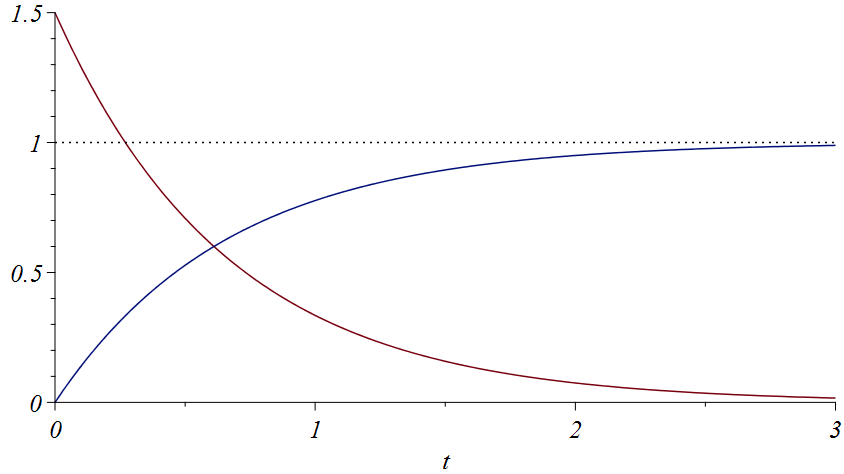
\includegraphics[width=0.7\textwidth]{images/exp-cum.png}
  \end{center}
\end{itemize}
\end{n}


\ssn{Foundations}
We will not present a completely rigorous version of the foundations of continuous probability. The fundamental difficulty is that an event will be a subset of the sample space and it needs to be a subset over which a suitable pdf can be integrated, and we do not study integration rigorously until later in the degree.  We will only consider events that are finite unions of intervals. 

Given that we assume that $f_X(x)$ is piecewise continuous,  $\int_x^x f_X(u) \dd u = 0$ and we are forced to have $\PP(X=x) = 0$ for all points $a$.   Consequently it does not matter if endpoints are included because $\PP(X<x) = \PP(X \leq x)$ and so on. 

We will assume that probabilities for events obey the fundamental properties in \S\ref{prprops} without proof.    
\end{n}
